\chapter{Neural networks (part 1): from the neuron to the MLP}\label{ch-06}

With neural networks we enter the heart of the course. This first part
starts from the biological inspiration, introduces the artificial
neuron and the \textbf{Perceptron} with its learning algorithm and the
\textbf{convergence theorem}, compares the Perceptron with LMS,
introduces sigmoidal activation functions and arrives at the
\textbf{Multi-Layer Perceptron} (MLP), analysed as a flexible function,
as an adaptive basis expansion and as a universal approximator. It
closes with the problems that learning in a network raises, which will
be solved by \textbf{backpropagation}.

\section{Neural networks as an ML
tool}\label{le-reti-neurali-come-strumento-di-ml}

Neural networks are studied with two different goals:

\begin{itemize}
\tightlist
\item
  \textbf{modelling biological systems} and learning processes
  (philosophy, psychology, neurobiology, cognitive science,
  computational neuroscience): here \textbf{biological realism} is
  essential;
\item
  \textbf{building effective ML systems and algorithms} (statistics,
  AI, physics, mathematics, engineering), often losing strict
  biological realism: here the \textbf{computational and algorithmic}
  properties matter.
\end{itemize}

In the course we are interested in \textbf{ANNs} (\emph{Artificial
Neural Networks}) as a \textbf{flexible ML tool}, in the sense of
function approximation: a network implements a mathematical function
\(h(\mathbf{x})\) with special properties.

Despite being a ``historical machine'', neural networks remain a
powerful approach:

\begin{itemize}
\tightlist
\item
  they learn from examples;
\item
  they are \textbf{universal approximators} (Cybenko's theorem):
  flexible approaches for arbitrary functions, including non-linear
  ones;
\item
  they handle noise and incomplete data, with performance that
  \textbf{degrades gracefully} under adverse conditions;
\item
  they deal with real and discrete data, for regression and
  classification;
\item
  they are not a single model but a \textbf{paradigm} (in the class of
  sub-symbolic approaches).
\end{itemize}

The underlying ``philosophy'' is \textbf{connectionism}: complex
(mental, behavioural) behaviours that \textbf{emerge} from the
interaction of many simple interconnected computational units.

\section{The biological inspiration}\label{lispirazione-biologica}

The human brain has more than \(10^{10}\) neurons, each with
\(10^4\)--\(10^5\) connections. A neuron responds in about one
millisecond, yet we recognise an image in about 0.1 seconds: at most a
hundred \textbf{serial} computation steps. It follows that the brain
must perform a \textbf{massively parallel} computation. (Note that
face recognition, so easy for us, is complex for conventional
computers.)

\begin{figure}[htbp]
\centering
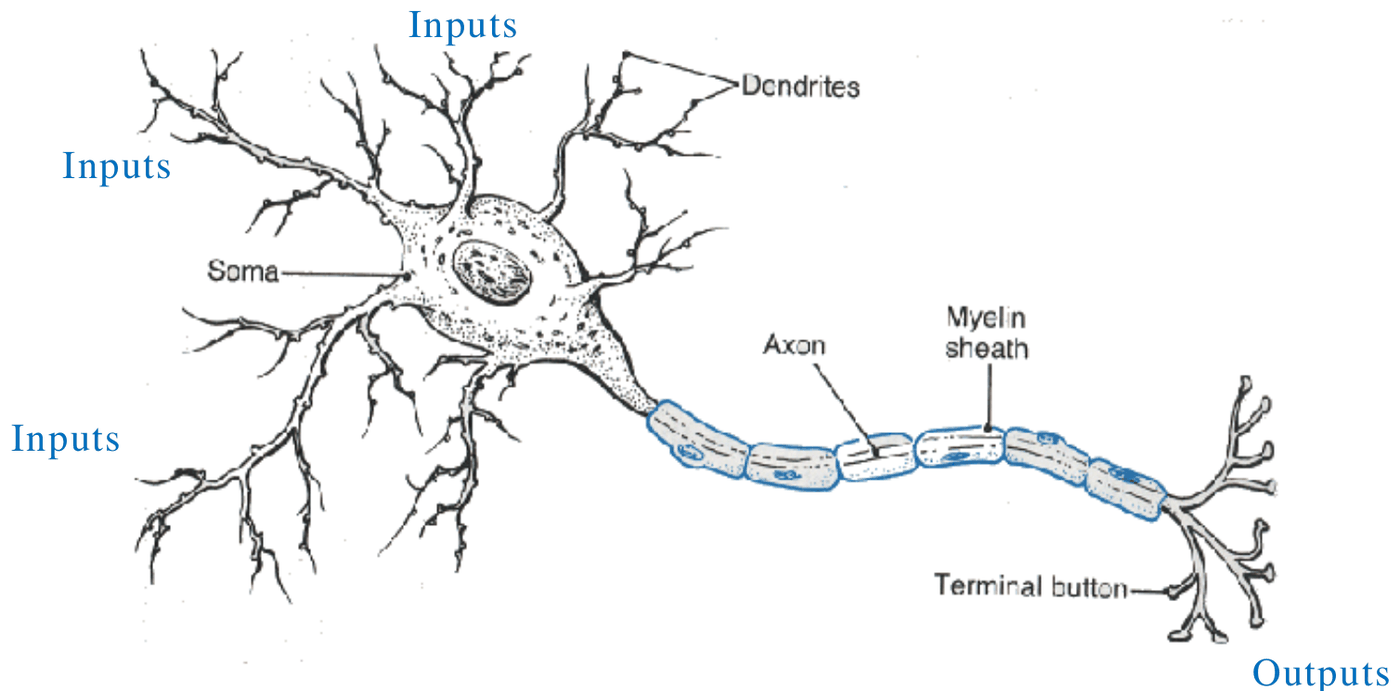
\includegraphics[width=0.80\linewidth,height=0.42\textheight,keepaspectratio]{images/06-nn1_neurone-biologico.png}
\caption{The biological neuron: dendrites (input), soma, axon and
terminals (output).}
\end{figure}

How it works, in short: the neuron goes through cycles of charge and
discharge (sodium and potassium ions); the inputs from the dendrites
modify the potential of the cell; once a \textbf{threshold} is
exceeded, a \textbf{spike} (a voltage pulse) is generated, and
information is also encoded in the time intervals between spikes.

The signal propagates along the axon up to the \textbf{synapses}, where
it passes (in chemical form, through \textbf{neurotransmitters}) to the
next neuron. Synapses can be \textbf{excitatory} or
\textbf{inhibitory}, and above all they change with learning: their
strength (the ``weight'') is reinforced in response to stimuli. This is
the \textbf{plasticity} of the nervous system.

\begin{boxdefinition}{Hebbian learning (Hebb, 1949)}

A synapse is strengthened when the inputs of the neuron (and the
correlated outputs) are repeated. The incoming stimulus reinforces the
synapse, hence \textbf{the weights move closer to the inputs}.

\end{boxdefinition}

\section{The artificial neuron}\label{il-neurone-artificiale}

\begin{figure}[htbp]
\centering
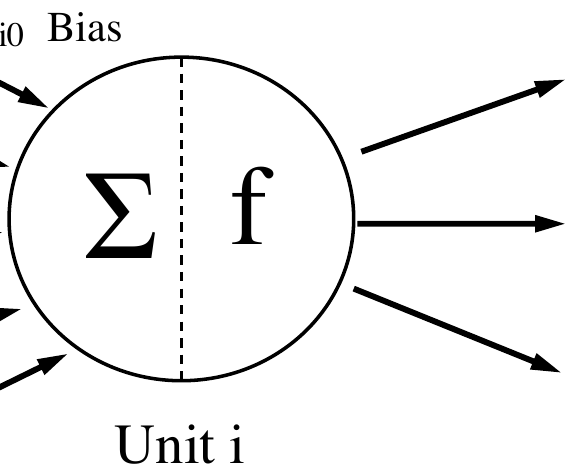
\includegraphics[width=0.43\linewidth,height=0.42\textheight,keepaspectratio]{images/06-nn1_unita.png}
\caption{The processing unit (artificial neuron).}
\end{figure}

A \textbf{unit} (node, neuron) receives inputs from external sources or
from other units. Each connection has a \textbf{weight} \(w\), a free
parameter that can be modified by learning (the analogue of synaptic
strength). Unit \(i\) computes: \[
net_i(\mathbf{x}) = \sum_j w_{ij}\, x_j, \qquad o_i(\mathbf{x}) = f\big(net_i(\mathbf{x})\big).
\]

\begin{itemize}
\tightlist
\item
  The weighted sum \(net_i\) is the \textbf{net input} of unit \(i\);
  it includes the bias \(w_{i0}\) through the constant input
  \(x_0 = 1\).
\item
  \(f\) is the \textbf{activation function} (linear, threshold,
  sigmoidal\ldots).
\end{itemize}

\begin{boxwarning}{Weight notation}

\(w_{ij}\) is the weight \textbf{of unit \(i\)}, i.e.\ of the
connection \textbf{from input/unit \(j\) to unit \(i\)} (not the other
way round). Some sources (for example Wikipedia in the section on
backpropagation, and some libraries) use the opposite convention; the
course always uses the traditional one: the first index is the
receiving unit.

\end{boxwarning}

Three classic activation functions:

\begin{figure}[htbp]
\centering
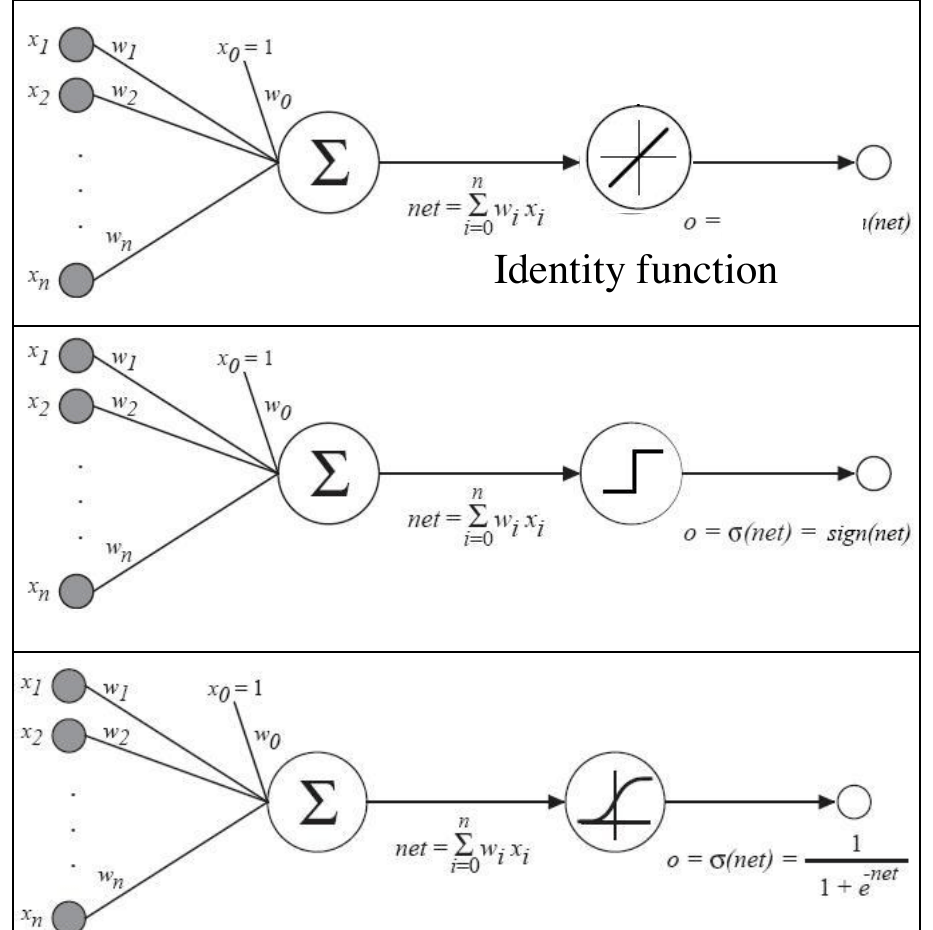
\includegraphics[width=0.54\linewidth,height=0.42\textheight,keepaspectratio]{images/06-nn1_attivazioni.png}
\caption{Linear (identity), threshold (Perceptron) and logistic (sigmoid)
activation functions.}
\end{figure}

\begin{enumerate}
\def\labelenumi{\arabic{enumi}.}
\tightlist
\item
  \textbf{linear} (identity): \(h(\mathbf{x}) = \sum_i w_i x_i\);
\item
  \textbf{threshold} (step): this is the \textbf{Perceptron}, i.e.\ the
  LTU already seen;
\item
  \textbf{logistic} (sigmoid): see later.
\end{enumerate}

\section{The Perceptron}\label{il-perceptron}

The \textbf{Perceptron} was proposed by Frank Rosenblatt (1957--1960)
for pattern classification, simulating human perception: an ``eye'' of
photocells connected to units that compute a weighted combination with
a threshold.

\begin{figure}[htbp]
\centering
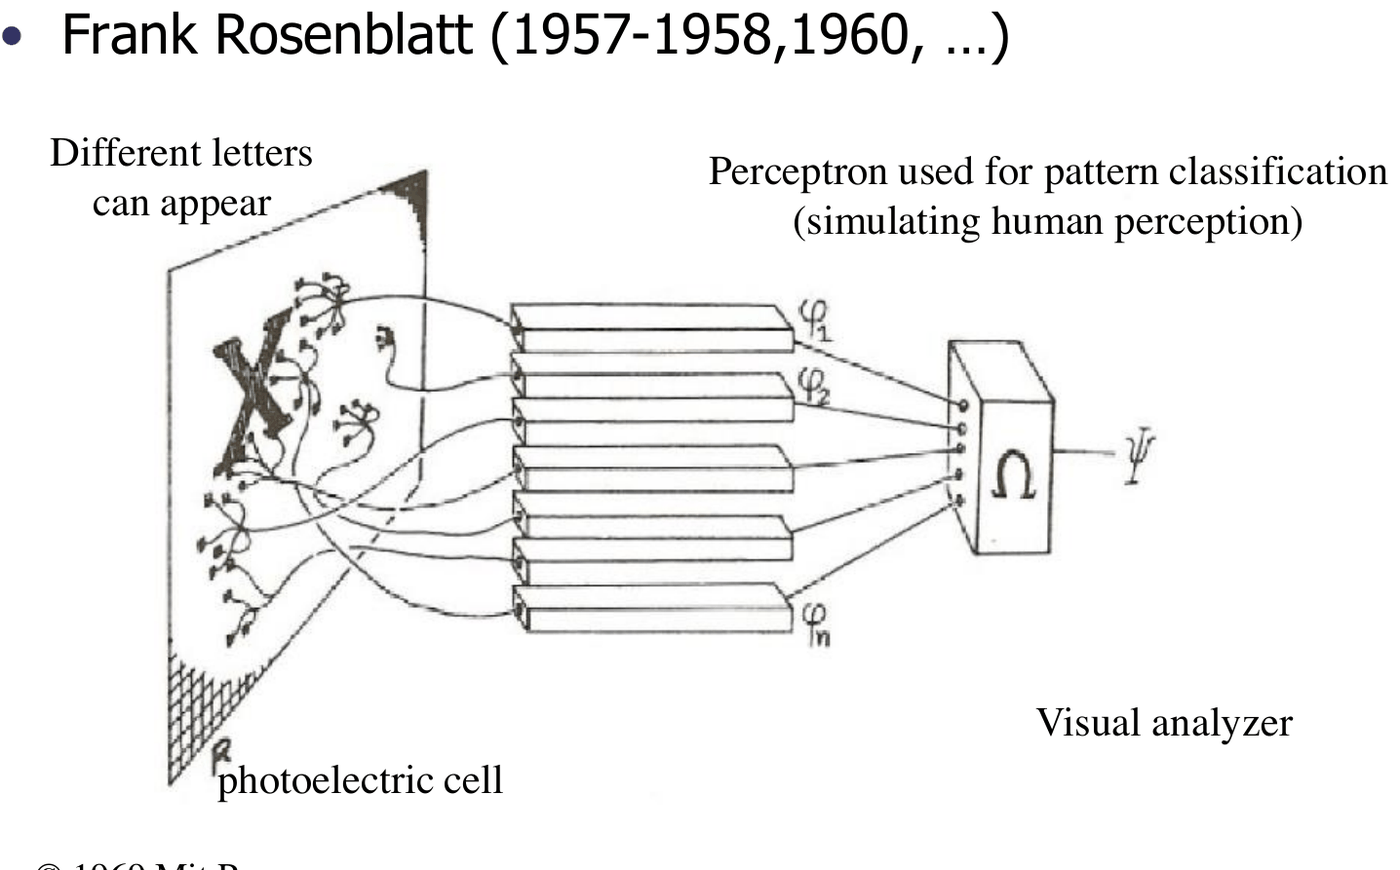
\includegraphics[width=0.63\linewidth,height=0.42\textheight,keepaspectratio]{images/06-nn1_perceptron-rosenblatt.png}
\caption{The original Perceptron, used to recognise letters.}
\end{figure}

The single neuron is a very simple computational unit. Minsky:
\emph{``for the kind of recognition it can do, it is such a simple
machine that it would be surprising if nature did not use it
somewhere''}. The Perceptron is a model of historical importance and
\textbf{paradigmatic} for the transition from linear to non-linear
models: by composing and connecting perceptrons one obtains
\textbf{MLP} networks (\emph{Multi-Layer Perceptron}).

\subsection{McCulloch and Pitts networks
(1943)}\label{le-reti-di-mcculloch-e-pitts-1943}

The first model, \emph{``A logical calculus of the ideas immanent in
nervous activity''} (1943), asked what a given network computes and
whether a network can compute a given logical formula.

\begin{itemize}
\tightlist
\item
  Neurons have two states: active (1) and inactive (0).
\item
  All synapses are equivalent and characterised by a real number (the
  strength \(w\)), positive for \textbf{excitatory} connections and
  negative for \textbf{inhibitory} ones.
\item
  A neuron \(i\) becomes active when the sum of the weights \(w_{ij}\)
  coming from the active neurons \(j\), plus a bias, exceeds zero.
\end{itemize}

Binary inputs and outputs: it is essentially the LTU/Perceptron.

\subsubsection{Representing Boolean
functions}\label{rappresentare-funzioni-booleane}

With \(net = \mathbf{w}^T\mathbf{x} = \sum_{i=0}^n w_i x_i\) and output
\(1\) if \(net > 0\), \(0\) (or \(-1\)) otherwise:

\begin{itemize}
\tightlist
\item
  \textbf{AND}: \(w_1 = w_2 = 1\), \(w_0 = -1.5\) (both inputs must be
  1 to exceed \(1.5\));
\item
  \textbf{OR}: \(w_1 = w_2 = 1\), \(w_0 = -0.5\) (one input at 1 is
  enough).
\end{itemize}

\begin{figure}[htbp]
\centering
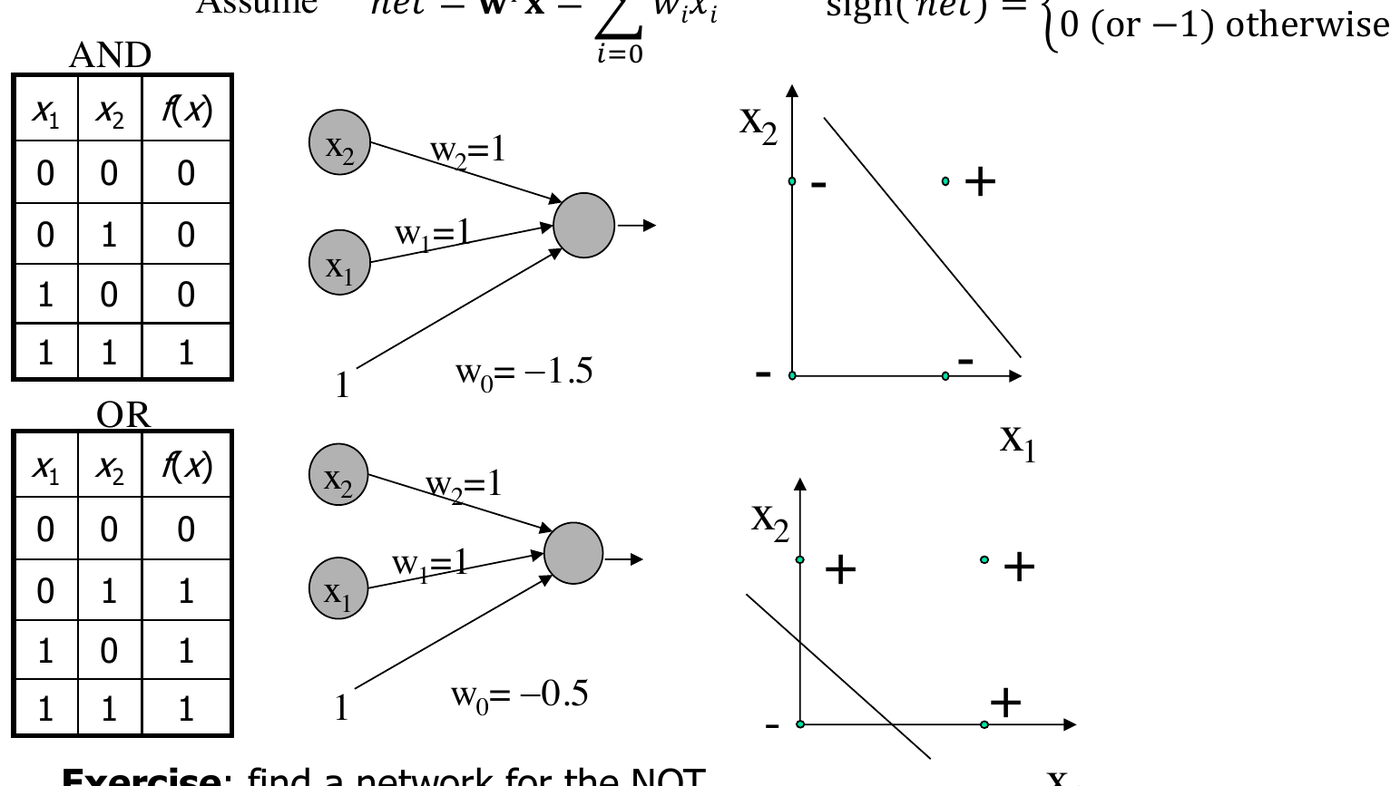
\includegraphics[width=0.80\linewidth,height=0.42\textheight,keepaspectratio]{images/06-nn1_and-or.png}
\caption{AND and OR implemented by a single perceptron.}
\end{figure}

(Exercise: NOT is obtained with \(w_1 = -1\), \(w_0 = 0.5\): for
\(x_1 = 0\) the net is \(0.5 > 0\), for \(x_1 = 1\) it is \(-0.5\).)

\subsubsection{XOR and two-layer
networks}\label{lo-xor-e-le-reti-a-due-strati}

\textbf{XOR} is not linearly separable: no single perceptron can
represent it (Minsky and Papert, 1969). It can however be decomposed:
\[
x_1 \oplus x_2 = x_1\bar{x}_2 + \bar{x}_1 x_2 = \bar{h}_1 \cdot h_2, \qquad \text{with } h_1 = x_1 \cdot x_2 \text{ (AND)}, \quad h_2 = x_1 + x_2 \text{ (OR)}.
\]

\begin{boxtheorem}{XOR as a composition of AND and OR}

By De Morgan,
\(\overline{h_1} = \overline{a \wedge b} = \bar a \vee \bar b\).
Hence \[
\bar h_1 \wedge h_2 = (\bar a \vee \bar b) \wedge (a \vee b) = (\bar a \wedge a) \vee (\bar a \wedge b) \vee (a \wedge \bar b) \vee (b \wedge \bar b) = (\bar a \wedge b) \vee (a \wedge \bar b) = a \oplus b.
\]

\end{boxtheorem}

We thus build a \textbf{two-layer} network: two hidden units compute
\(h_1\) (AND) and \(h_2\) (OR), and an output unit computes
\(\bar h_1 \wedge h_2\) (weights \(-1\) from \(h_1\) and \(+1\) from
\(h_2\), bias \(-0.5\)).

\begin{figure}[htbp]
\centering
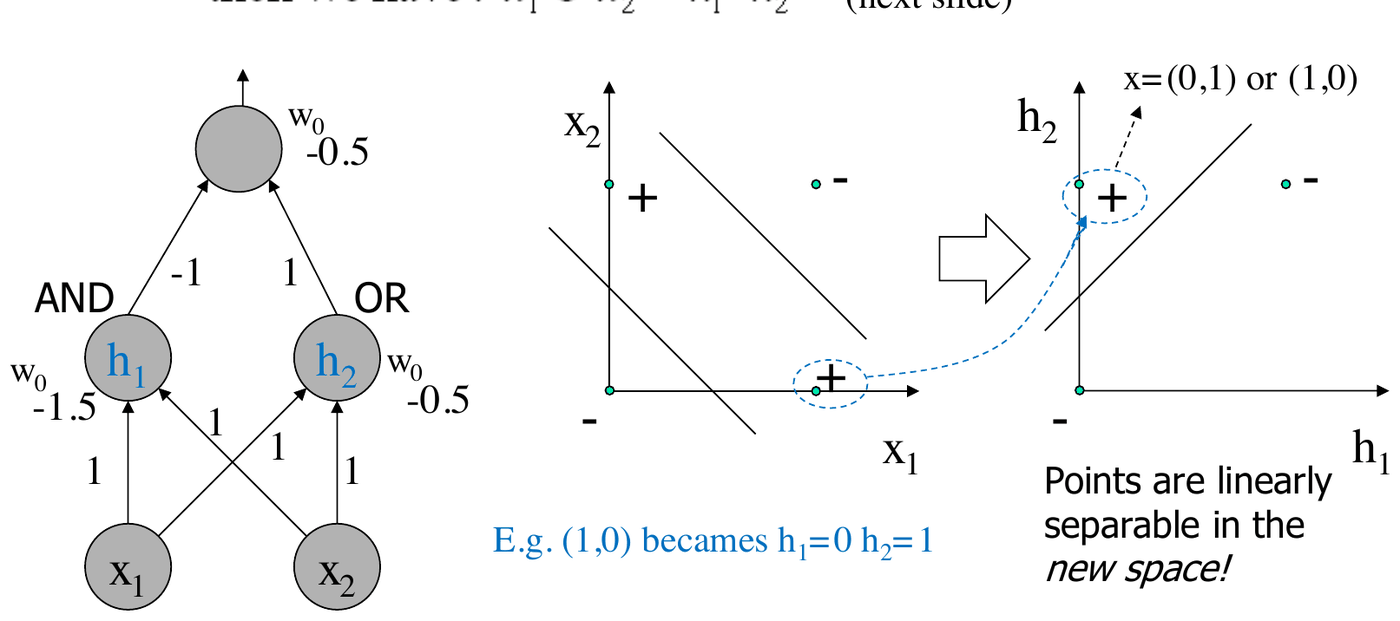
\includegraphics[width=0.89\linewidth,height=0.42\textheight,keepaspectratio]{images/06-nn1_xor-rete.png}
\caption{XOR with a two-layer network: in the space of the hidden units
\((h_1, h_2)\) the points become linearly separable.}
\end{figure}

\subsection{The hidden layer as a
representation}\label{lo-strato-nascosto-come-rappresentazione}

The figure shows the key concept: the hidden layer produces an
\textbf{internal re-representation} of the inputs. The point \((1,0)\),
which in the original space lies in the bottom-right corner, becomes
\(h_1 = 0\), \(h_2 = 1\): the two positive points \((0,1)\) and
\((1,0)\) are mapped \textbf{to the same point} \((0,1)\) of the
hidden space, and the problem becomes linearly separable for the output
unit.

\begin{boxtip}{The most important concept of neural networks}

Developing \textbf{high-level features} in the hidden layers is the key
factor of neural networks: the representation in the hidden layer
makes the task of the output layer easier. This composition of
intermediate operations can be extended over \textbf{many layers of
abstraction}, and --- unlike what we saw here, where the weights are
chosen by hand --- in neural networks these representations \textbf{are
learned}. This is the idea behind \emph{representation learning} and
\textbf{deep learning}.

\end{boxtip}

\begin{boxabstract}{Properties of perceptron networks}

\begin{itemize}
\tightlist
\item
  Perceptrons represent AND, OR, NOT (and hence NAND, NOR) →
  \textbf{every Boolean function} can be represented by a network of
  perceptrons.
\item
  \textbf{Two levels} are enough (more levels can be more efficient).
\item
  A single layer is not enough (Minsky and Papert, 1969): limits due
  to linear separability.
\item
  So far, however, \textbf{we have no learning algorithm}, not even for
  a single unit.
\end{itemize}

\end{boxabstract}

\section{Learning for a single
unit}\label{apprendimento-per-una-singola-unituxe0}

Historically there are two families of methods:

\begin{enumerate}
\def\labelenumi{\arabic{enumi}.}
\tightlist
\item
  \textbf{Adaline} (\emph{Adaptive Linear Neuron}, Widrow and Hoff):
  during training the unit is \textbf{linear}; the direct LMS solution
  or gradient descent is used (exactly as in the lecture on linear
  models). It serves for regression and, with the threshold,
  classification. It is the approach we will generalise to MLPs.
\item
  \textbf{Perceptron} (Rosenblatt): during training the unit is
  \textbf{non-linear} (with a threshold function). Classification only;
  its capabilities and convergence are studied.
\end{enumerate}

To build a linear classifier we thus have three algorithms: direct LMS,
gradient LMS and now the Perceptron algorithm (and others will come,
such as SVMs).

\subsection{The Perceptron learning
algorithm}\label{lalgoritmo-di-apprendimento-del-perceptron}

The goal is to \textbf{minimise the number of misclassified patterns}:
find \(\mathbf{w}\) such that
\(\operatorname{sign}(\mathbf{w}^T\mathbf{x}) = d\). It is an
\textbf{on-line} algorithm (one step per pattern).

\begin{boxabstract}{Perceptron Learning Algorithm}

\begin{enumerate}
\def\labelenumi{\arabic{enumi}.}
\tightlist
\item
  Initialise the weights (to zero or to small random values).
\item
  Choose a learning rate \(\eta \in (0, 1)\).
\item
  Until the stopping condition is met (e.g.\ the weights no longer
  change), for each pattern \((\mathbf{x}, d)\) with
  \(d \in \{+1, -1\}\):

  \begin{itemize}
  \tightlist
  \item
    compute \(out = \operatorname{sign}(\mathbf{w}^T\mathbf{x})\);
  \item
    if \(out = d\), \textbf{do not change the weights};
  \item
    if \(out \ne d\), update:
    \(\mathbf{w}_{new} = \mathbf{w} + \eta\, d\, \mathbf{x}\).
  \end{itemize}
\end{enumerate}

\end{boxabstract}

In practice \(\eta\mathbf{x}\) is added if
\(\mathbf{w}^T\mathbf{x} \le 0\) and \(d = +1\) (false negative), and
\(\eta\mathbf{x}\) is subtracted if \(\mathbf{w}^T\mathbf{x} > 0\) and
\(d = -1\) (false positive). Equivalently: \[
\mathbf{w}_{new} = \mathbf{w} + \tfrac{1}{2}\eta\,(d - out)\,\mathbf{x},
\] because \(d - out\) is \(0\) if the classification is correct and
\(\pm 2\) if it is wrong.

\begin{boxwarning}{Difference from LMS}

The formula looks like the LMS one, but here \(out\) contains the
\textbf{sign}: \(out = \operatorname{sign}(\mathbf{w}^T\mathbf{x})\),
whereas in LMS the error was computed on \(\mathbf{w}^T\mathbf{x}\)
(without threshold).

\end{boxwarning}

\subsubsection{Geometric view}\label{vista-geometrica}

\begin{figure}[htbp]
\centering
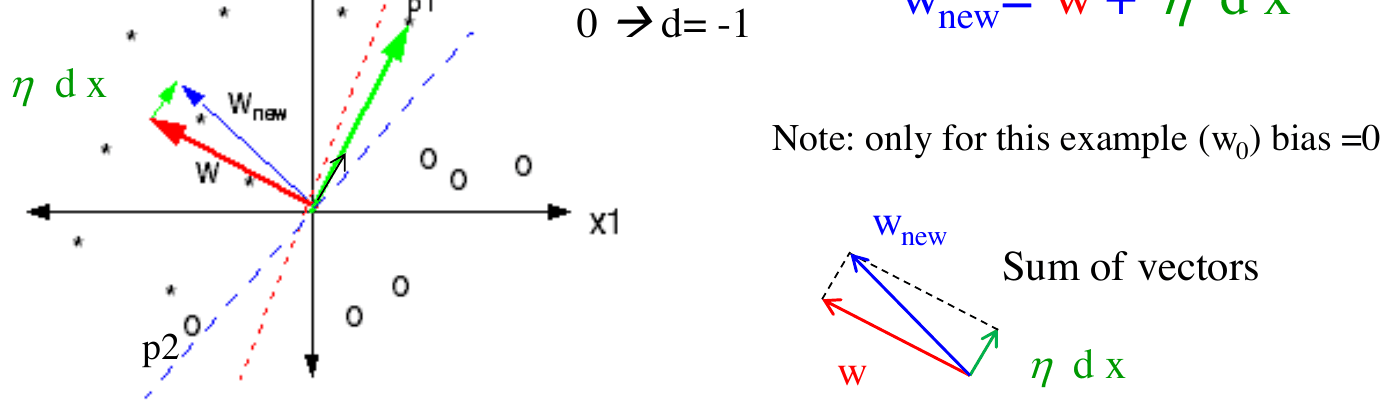
\includegraphics[width=0.86\linewidth,height=0.42\textheight,keepaspectratio]{images/06-nn1_perceptron-geometria.png}
\caption{Perceptron update: \(\mathbf{w}\) is moved in the direction of
the misclassified pattern \(p_1\).}
\end{figure}

Before the update \(\mathbf{w}\) (which points towards the positive
region) misclassifies both \(p_1\) and \(p_2\). Choosing \(p_1\), which
has target \(d = +1\), \(\mathbf{w}\) is moved a little in the
direction of \(p_1\) (vector sum \(\mathbf{w} + \eta d\mathbf{x}\)),
and the new boundary is better. (Exercise: if \(p_2\) is chosen, with
\(d = -1\), \(\mathbf{w}\) is moved away from \(p_2\).)

\subsection{Delta rule: two readings}\label{delta-rule-due-letture}

\begin{itemize}
\tightlist
\item
  The form \(\mathbf{w}_{new} = \mathbf{w} + \eta\, d\,\mathbf{x}\) can
  be read as \textbf{Hebbian learning}: \(\mathbf{w}\) moves towards
  \(\mathbf{x}\).
\item
  The form
  \(\mathbf{w}_{new} = \mathbf{w} + \eta\,(d - out)\,\mathbf{x} = \mathbf{w} + \eta\,\delta\,\mathbf{x}\)
  is an \textbf{error-correction} rule (delta rule, Widrow-Hoff): the
  weight changes in proportion to the error.
\end{itemize}

In terms of neurons: \emph{the change of a synaptic weight is
proportional to the product of the error signal and the input signal
that excites the synapse}. The computation is easy when the error
signal \(\delta\) is \textbf{directly measurable}, i.e.\ when we know
the desired response for the unit. (This will be the problem in
networks with hidden layers.)

\subsection{Representing and
learning}\label{rappresentare-e-apprendere}

The Perceptron can \textbf{represent} linear decision boundaries, so it
solves linearly separable problems. But can it always \textbf{learn}
the solution? Yes: the Perceptron with its algorithm is always able to
learn what it can represent.

\begin{boxnote}{A historical result}

The convergence theorem is a milestone: a \textbf{biologically
inspired} model, with well-defined and \textbf{mathematically proven}
computational capabilities.

\end{boxnote}

\subsection{The Perceptron convergence
theorem}\label{il-teorema-di-convergenza-del-perceptron}

\begin{boxtheorem}{Perceptron convergence theorem}

If the problem is \textbf{linearly separable}, the Perceptron algorithm
converges (correctly classifying all patterns) in a \textbf{finite
number of steps}, regardless of the starting point (although the final
solution is not unique and depends on the starting point).

If the problem is not separable, the algorithm can be unstable: it
develops \textbf{cycles}, with weights that are not necessarily
optimal.

\end{boxtheorem}

In the proof we omit the \(T\) in dot products between vectors.

\subsubsection{Preliminaries 1: reducing to all-positive
patterns}\label{preliminari-1-ridursi-a-pattern-tutti-positivi}

Let \((\mathbf{x}_i, d_i)\) be the training examples,
\(d_i \in \{+1, -1\}\), \(i = 1,\dots,l\). If the problem is linearly
separable there exists a solution \(\mathbf{w}^*\) such that \[
d_i(\mathbf{w}^*\mathbf{x}_i) \ge \alpha, \qquad \text{with } \alpha = \min_i d_i(\mathbf{w}^*\mathbf{x}_i) > 0.
\] Hence \(\mathbf{w}^*(d_i\mathbf{x}_i) \ge \alpha\). Defining
\(\mathbf{x}'_i = d_i\mathbf{x}_i\), \textbf{\(\mathbf{w}^*\) is a
solution of the original problem if and only if it is a solution of the
problem \((\mathbf{x}'_i, +1)\)} with all positive targets:

\begin{itemize}
\tightlist
\item
  (if) \(\mathbf{w}^*\) solves the original problem
  \(\Rightarrow d_i(\mathbf{w}^*\mathbf{x}_i) \ge \alpha \Rightarrow \mathbf{w}^*\mathbf{x}'_i \ge \alpha \Rightarrow \mathbf{w}^*\)
  solves \((\mathbf{x}'_i, +1)\);
\item
  (only if) the reverse reasoning.
\end{itemize}

It is therefore enough to prove the theorem for a problem with
\textbf{only positive patterns}: ``flipping'' the negative patterns
changes nothing.

\subsubsection{\texorpdfstring{Preliminaries 2: form of the weights
after \(q\) errors}{Preliminaries 2: form of the weights after q errors}}\label{preliminari-2-forma-dei-pesi-dopo-q-errori}

Assume \(\mathbf{w}(0) = \mathbf{0}\), \(\eta = 1\) and define
\(\beta = \max_i \|\mathbf{x}_i\|^2\). With only positive patterns, the
rule becomes \(\mathbf{w}(j) = \mathbf{w}(j-1) + \mathbf{x}_{i_j}\) at
each error. After \(q\) errors (all false negatives): \[
\mathbf{w}(q) = \sum_{j=1}^{q} \mathbf{x}_{i_j},
\] where \(i_j\) denotes the misclassified patterns (for example
indices 2, 8, 9, 14 of the training set; the same pattern can appear
several times).

\subsubsection{Proof idea}\label{idea-della-dimostrazione}

We find a \textbf{lower bound} on \(\|\mathbf{w}(q)\|^2\) that grows
as \(q^2\) and an \textbf{upper bound} that grows as \(q\). Since a
quadratic function sooner or later exceeds a linear one, the two
bounds are compatible only for \(q\) up to a certain maximum value: the
number of errors (and thus of updates) is finite.

\begin{figure}[htbp]
\centering
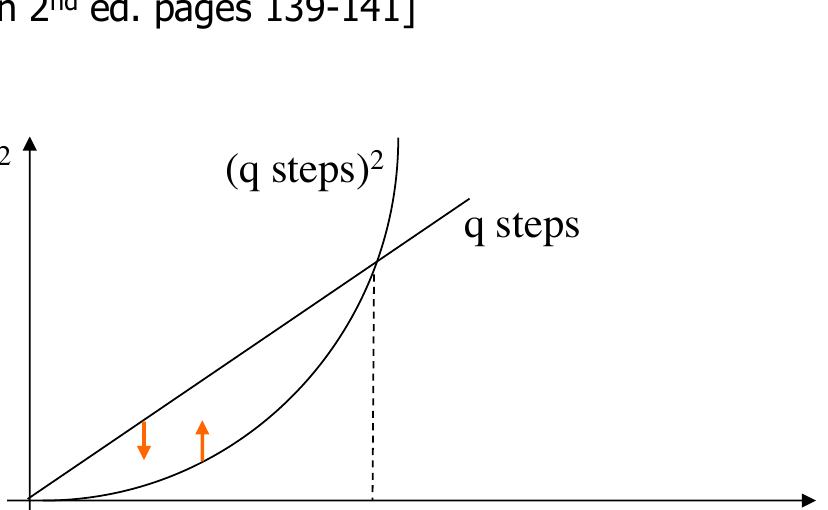
\includegraphics[width=0.54\linewidth,height=0.42\textheight,keepaspectratio]{images/06-nn1_convergenza.png}
\caption{Proof idea: the quadratic lower bound and the linear upper bound
meet at \(q_{max}\).}
\end{figure}

\subsubsection{Lower bound}\label{limite-inferiore}

\[
\mathbf{w}^{*T}\mathbf{w}(q) = \mathbf{w}^{*T}\sum_{j=1}^{q}\mathbf{x}_{i_j} \ge q\alpha,
\] because each term \(\mathbf{w}^{*T}\mathbf{x}_{i_j}\) is at least
\(\alpha\). By the \textbf{Cauchy-Schwarz inequality},
\(\|\mathbf{a}\|^2\|\mathbf{b}\|^2 \ge (\mathbf{a}^T\mathbf{b})^2\);
with \(\mathbf{a} = \mathbf{w}^*\) and \(\mathbf{b} = \mathbf{w}(q)\):
\[
\|\mathbf{w}^*\|^2\,\|\mathbf{w}(q)\|^2 \ge \big(\mathbf{w}^{*T}\mathbf{w}(q)\big)^2 \ge (q\alpha)^2 \quad\Rightarrow\quad \|\mathbf{w}(q)\|^2 \ge \frac{(q\alpha)^2}{\|\mathbf{w}^*\|^2}.
\]

\subsubsection{Upper bound}\label{limite-superiore}

Using
\(\|\mathbf{a} + \mathbf{b}\|^2 = \|\mathbf{a}\|^2 + 2\mathbf{a}\mathbf{b} + \|\mathbf{b}\|^2\):
\[
\|\mathbf{w}(q)\|^2 = \|\mathbf{w}(q-1) + \mathbf{x}_{i_q}\|^2 = \|\mathbf{w}(q-1)\|^2 + 2\,\mathbf{w}(q-1)\,\mathbf{x}_{i_q} + \|\mathbf{x}_{i_q}\|^2.
\] Since \(\mathbf{x}_{i_q}\) was misclassified (it is the \(q\)-th
error), \(\mathbf{w}(q-1)\,\mathbf{x}_{i_q} \le 0\): dropping this
non-positive term we get \[
\|\mathbf{w}(q)\|^2 \le \|\mathbf{w}(q-1)\|^2 + \|\mathbf{x}_{i_q}\|^2,
\] and iterating (with \(\mathbf{w}(0) = \mathbf{0}\)): \[
\|\mathbf{w}(q)\|^2 \le \sum_{j=1}^{q}\|\mathbf{x}_{i_j}\|^2 \le q\beta.
\]

\subsubsection{Conclusion}\label{conclusione}

Putting the two bounds together: \[
q\beta \;\ge\; \|\mathbf{w}(q)\|^2 \;\ge\; \frac{(q\alpha)^2}{\|\mathbf{w}^*\|^2} \quad\Rightarrow\quad q \le \frac{\beta\,\|\mathbf{w}^*\|^2}{\alpha^2}.
\] The number of errors (and thus of updates) is bounded by a
constant: the algorithm converges in a \textbf{finite number of
steps}. \(\blacksquare\)

\begin{boxtip}{Interpretation of the bound}

The number of steps grows with \(\beta\) (how ``large'' the patterns
are) and decreases with \(\alpha^2\): \(\alpha\) measures how ``well
separated'' the problem is (the minimum margin of the solution
\(\mathbf{w}^*\)). Problems with classes close to the separating
hyperplane require more steps. The idea of \textbf{margin} will become
central in SVMs.

\end{boxtip}

\section{Perceptron versus LMS}\label{perceptron-contro-lms}

The two rules look similar
(\(\mathbf{w}_{new} = \mathbf{w} + \eta\,\delta\,\mathbf{x}\)), but:

\begin{itemize}
\tightlist
\item
  LMS is derived (through the gradient) \textbf{without} the threshold
  function, minimising the error of the linear unit:
  \(\delta = d - \mathbf{w}^T\mathbf{x}\);
\item
  the Perceptron uses the thresholded output:
  \(\delta = d - \operatorname{sign}(\mathbf{w}^T\mathbf{x})\).
\end{itemize}

Of course the model trained with LMS can be used to classify by
applying the threshold
(\(h(\mathbf{x}) = \operatorname{sign}(\mathbf{w}^T\mathbf{x})\),
LTU).

An important consequence: \textbf{LMS can misclassify even linearly
separable problems}. LMS does not minimise the number of errors of the
LTU, but the squared error, and it modifies the weights \textbf{even
for patterns already classified correctly}. A correct pattern that is
``far'' from the hyperplane (with \(\mathbf{w}^T\mathbf{x}\) much
larger than 1) still produces a large squared error that ``pulls'' the
hyperplane.

\begin{figure}[htbp]
\centering
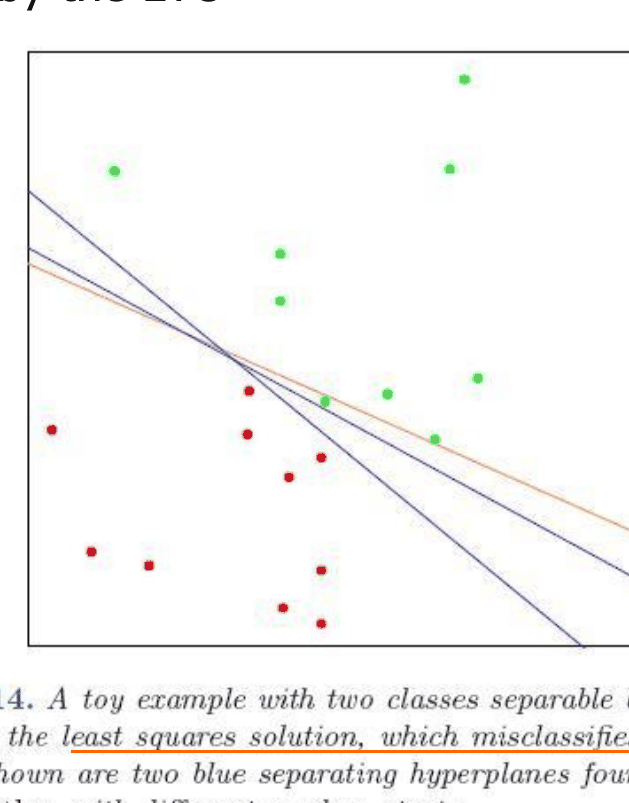
\includegraphics[width=0.43\linewidth,height=0.42\textheight,keepaspectratio]{images/06-nn1_lms-vs-perc.png}
\caption{A separable problem: the LMS solution (orange) misclassifies
one point, the Perceptron (blue, two different initialisations)
separates everything (Hastie et al., Fig.\ 4.14).}
\end{figure}

{\def\LTcaptype{none} % do not increment counter
\begin{longtable}[]{@{}
  >{\raggedright\arraybackslash}p{(\linewidth - 2\tabcolsep) * \real{0.5000}}
  >{\raggedright\arraybackslash}p{(\linewidth - 2\tabcolsep) * \real{0.5000}}@{}}
\toprule\noalign{}
\begin{minipage}[b]{\linewidth}\raggedright
Perceptron Learning Algorithm
\end{minipage} & \begin{minipage}[b]{\linewidth}\raggedright
LMS
\end{minipage} \\
\midrule\noalign{}
\endhead
\bottomrule\noalign{}
\endlastfoot
Minimises misclassifications
(\(out = \operatorname{sign}(\mathbf{w}^T\mathbf{x})\)) & Minimises
\(E(\mathbf{w})\) with \(out = \mathbf{w}^T\mathbf{x}\) \\
Always converges for separable problems, in a finite number of steps,
to a perfect classifier & \textbf{Asymptotic} convergence, also for
non-separable problems \\
Does not converge if the problem is not separable & Not always zero
classification errors, even on separable problems \\
Hard to extend to networks of units & \textbf{Extendable to networks}
with the gradient approach \\
\end{longtable}
}

The last row is decisive: to build neural networks we need a
\textbf{gradient}-based approach, which requires differentiable
functions.

\section{Sigmoidal activation
functions}\label{funzioni-di-attivazione-sigmoidali}

Besides the linear and threshold functions, \textbf{non-linear
``squashing''} functions are used, such as the \textbf{logistic
sigmoid}, which takes continuous values in the bounded interval
\([0,1]\): \[
f_\sigma(x) = \frac{1}{1 + e^{-ax}}.
\] It is a \textbf{smooth and differentiable version of the threshold
function}. The parameter \(a\) is the \textbf{slope}.

\begin{figure}[htbp]
\centering
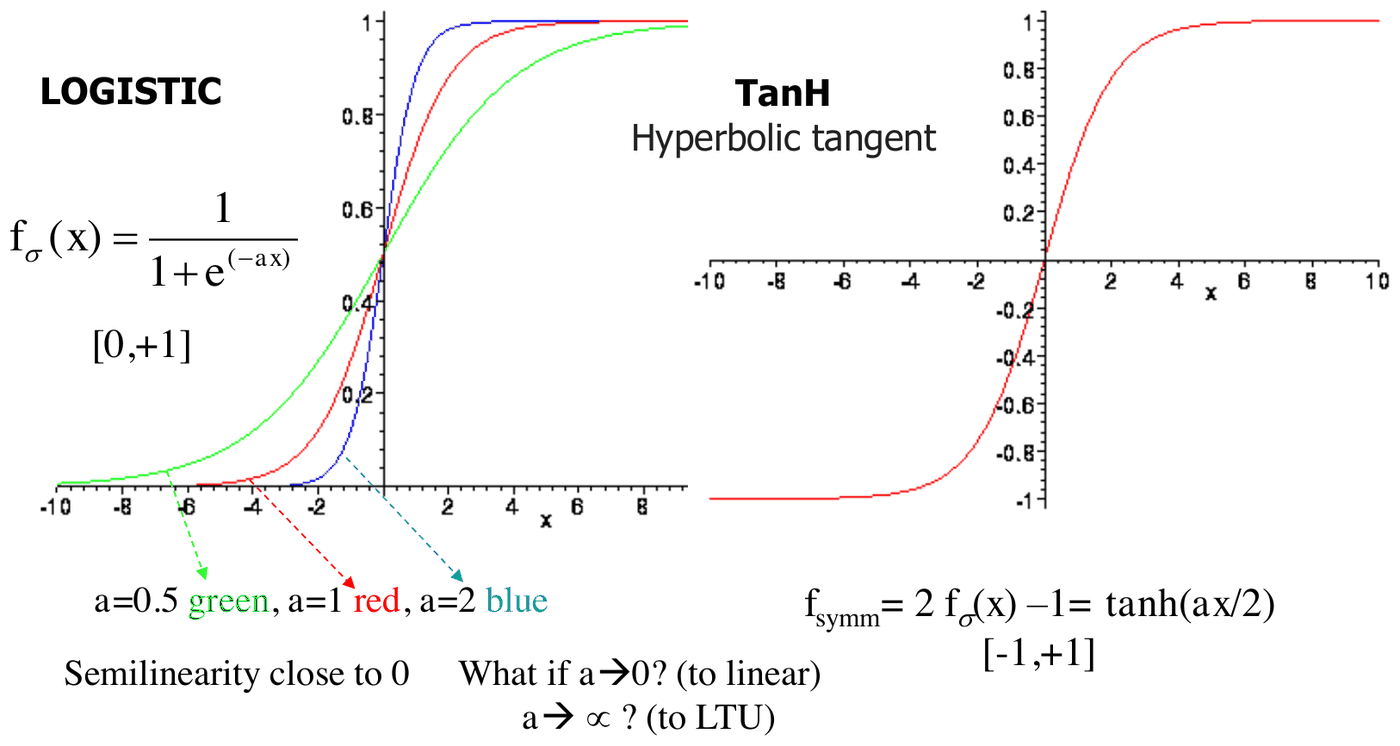
\includegraphics[width=0.91\linewidth,height=0.42\textheight,keepaspectratio]{images/06-nn1_sigmoidi.png}
\caption{Logistic sigmoid (left) for different values of \(a\) and
hyperbolic tangent (right).}
\end{figure}

The symmetric version is the \textbf{hyperbolic tangent}, with values
in \([-1, +1]\): \[
f_{symm}(x) = 2f_\sigma(x) - 1 = \tanh(ax/2).
\]

Near zero the sigmoid is almost linear (\textbf{semi-linearity}). As
\(a\) varies:

\begin{itemize}
\tightlist
\item
  for \(a \to 0\) the function tends to a \textbf{linear} function
  (very flat);
\item
  for \(a \to \infty\) it tends to the \textbf{step} function (LTU).
\end{itemize}

For classification, with the logistic function an output \(\ge 0.5\)
corresponds to the positive class and \(< 0.5\) to the zero/negative
class (for tanh the threshold is 0). The threshold can be moved
(studying the effect on false positives/negatives or with a ROC curve),
and a \textbf{rejection zone} can also be defined around the threshold
to avoid fragile decisions.

\subsection{Other activation
functions}\label{altre-funzioni-di-attivazione}

\begin{itemize}
\tightlist
\item
  \textbf{Radial basis functions} (RBF): \(f(x) = e^{-ax^2}\) applied
  to \(\|\mathbf{w} - \mathbf{x}_{input}\|\), i.e.\ a Gaussian centred
  on the weights → \textbf{RBF networks}.
\item
  \textbf{Softmax}: for the case with multiple outputs (see later
  lectures).
\item
  \textbf{Stochastic neurons}: output \(+1\) with probability
  \(P(net)\), \(-1\) otherwise → \textbf{Boltzmann machines} and
  statistical mechanics models.
\item
  \textbf{Piecewise linear} approximations of tanh, for efficient
  computation (even with binary shifts).
\item
  \textbf{ReLU} (\emph{Rectified Linear Unit}): \(f(x) = \max(0, x)\).
  It has become the default choice for deep models; it will be
  discussed in deep learning.
\item
  \textbf{Softplus}, its smooth approximation:
  \(f(x) = \ln(1 + e^x)\).
\end{itemize}

Many activation functions have similar performance in practice.

\subsection{Derivatives}\label{derivate}

\begin{itemize}
\tightlist
\item
  The derivative of the identity is 1.
\item
  The derivative of the step function is \textbf{not defined} (at zero)
  and is zero elsewhere: this is exactly why it is not used with LMS.
\item
  For sigmoids (with \(a = 1\)): \[
  \frac{df_\sigma(x)}{dx} = f_\sigma(x)\big(1 - f_\sigma(x)\big), \qquad \frac{d\tanh(x)}{dx} = 1 - \tanh^2(x).
  \] (With generic \(a\):
  \(\frac{df_\sigma}{dx} = a\,f_\sigma(x)(1 - f_\sigma(x))\).)
\end{itemize}

\begin{boxnote}{Derivation of the derivative of the logistic}

\(f_\sigma(x) = (1 + e^{-x})^{-1}\), hence
\(f'_\sigma(x) = \frac{e^{-x}}{(1 + e^{-x})^2} = \frac{1}{1 + e^{-x}} \cdot \frac{e^{-x}}{1 + e^{-x}} = f_\sigma(x)\big(1 - f_\sigma(x)\big)\),
because \(\frac{e^{-x}}{1 + e^{-x}} = 1 - \frac{1}{1 + e^{-x}}\). It
is convenient: the derivative is computed from the value of the
function itself.

\end{boxnote}

\subsection{LMS with a sigmoidal
unit}\label{lms-con-ununituxe0-sigmoidale}

Since the logistic is a smooth and differentiable threshold, we can
derive an LMS algorithm by computing the gradient of the squared error
as for linear units: we go from
\(o(\mathbf{x}) = \mathbf{x}^T\mathbf{w}\) to
\(o(\mathbf{x}) = f_\sigma(\mathbf{x}^T\mathbf{w})\), and minimise \[
E(\mathbf{w}) = \sum_{p=1}^{l}\big(d_p - f_\sigma(\mathbf{x}_p^T\mathbf{w})\big)^2.
\]

The gradient is obtained with the \textbf{chain rule},
\(\frac{\partial f}{\partial x} = \frac{\partial f}{\partial g}\frac{\partial g}{\partial x}\),
using as auxiliary variables \(g = net\) and then \(g = out\). For a
pattern \(p\) with \(net_p = \mathbf{x}_p^T\mathbf{w}\): \[
\frac{\partial E_p}{\partial w_j} = \frac{\partial E_p}{\partial o_p}\cdot\frac{\partial o_p}{\partial net_p}\cdot\frac{\partial net_p}{\partial w_j} = -2(d_p - o_p)\cdot f'_\sigma(net_p)\cdot x_{p,j}.
\] Summing over all patterns: \[
\frac{\partial E(\mathbf{w})}{\partial w_j} = -2\sum_{p=1}^{l}\big(d_p - o(\mathbf{x}_p)\big)\, f'_\sigma(net(\mathbf{x}_p))\; x_{p,j} = -2\sum_{p=1}^{l}\delta_p\, x_{p,j}.
\] This derivative answers the question: \textbf{how much does a
change in \(w_j\) affect the change in \(E\)?}

Gradient descent is identical to that for the linear unit, with a new
delta: \[
\mathbf{w}_{new} = \mathbf{w} + \eta\,\delta_p\,\mathbf{x}_p, \qquad \delta_p = \big(d_p - o(\mathbf{x}_p)\big)\, f'_\sigma(net(\mathbf{x}_p)).
\]

\begin{figure}[htbp]
\centering
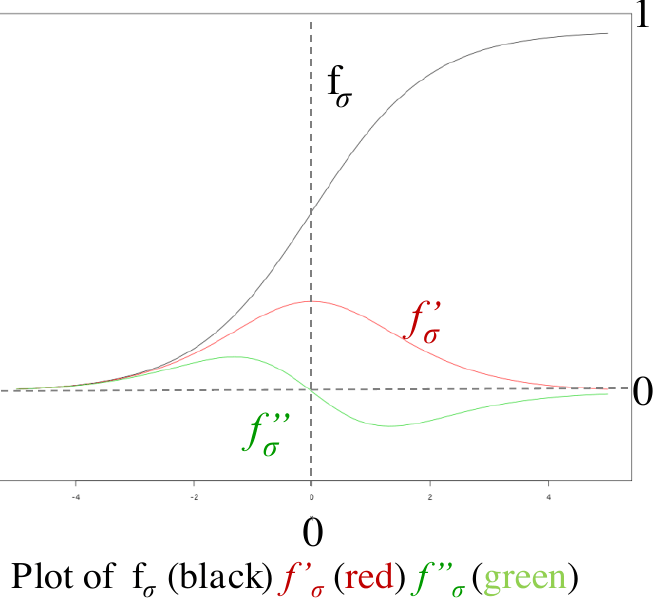
\includegraphics[width=0.43\linewidth,height=0.42\textheight,keepaspectratio]{images/06-nn1_derivate-sigmoide.png}
\caption{The logistic \(f_\sigma\) (black), its derivative \(f'_\sigma\)
(red) and the second derivative \(f''_\sigma\) (green).}
\end{figure}

It is still an \textbf{error-correction} rule, with some remarks:

\begin{itemize}
\tightlist
\item
  the slope \(a\) affects the size of the descent step;
\item
  \(f'_\sigma\) is \textbf{maximal for \(net\) close to 0} (almost
  linear zone): there the deltas can be large;
\item
  \(f'_\sigma\) is \textbf{minimal in saturated cases} (\(f\) close to
  0 or 1): small deltas, weights that change very slowly. One must
  \textbf{avoid premature saturation}, for example by \textbf{starting
  with small weights}.
\end{itemize}

\begin{boxtip}{A bridge between LMS and Perceptron}

When a pattern is classified correctly ``with confidence'' (output
saturated close to the target), \(f'_\sigma \approx 0\) and the
correction is almost zero, just as in the Perceptron, which does not
correct correct patterns. Using \(f_\sigma\) therefore approximates not
only the LTU, but also the Perceptron algorithm.

\end{boxtip}

\section{Neural networks: the Multi-Layer
Perceptron}\label{le-reti-neurali-il-multi-layer-perceptron}

All the ingredients are ready. An \textbf{MLP} can be seen in two
ways:

\begin{itemize}
\tightlist
\item
  \textbf{A.} as a \textbf{network of interconnected units};
\item
  \textbf{B.} as a \textbf{flexible function} \(h(\mathbf{x})\),
  composed of nested non-linear functions.
\end{itemize}

\begin{figure}[htbp]
\centering
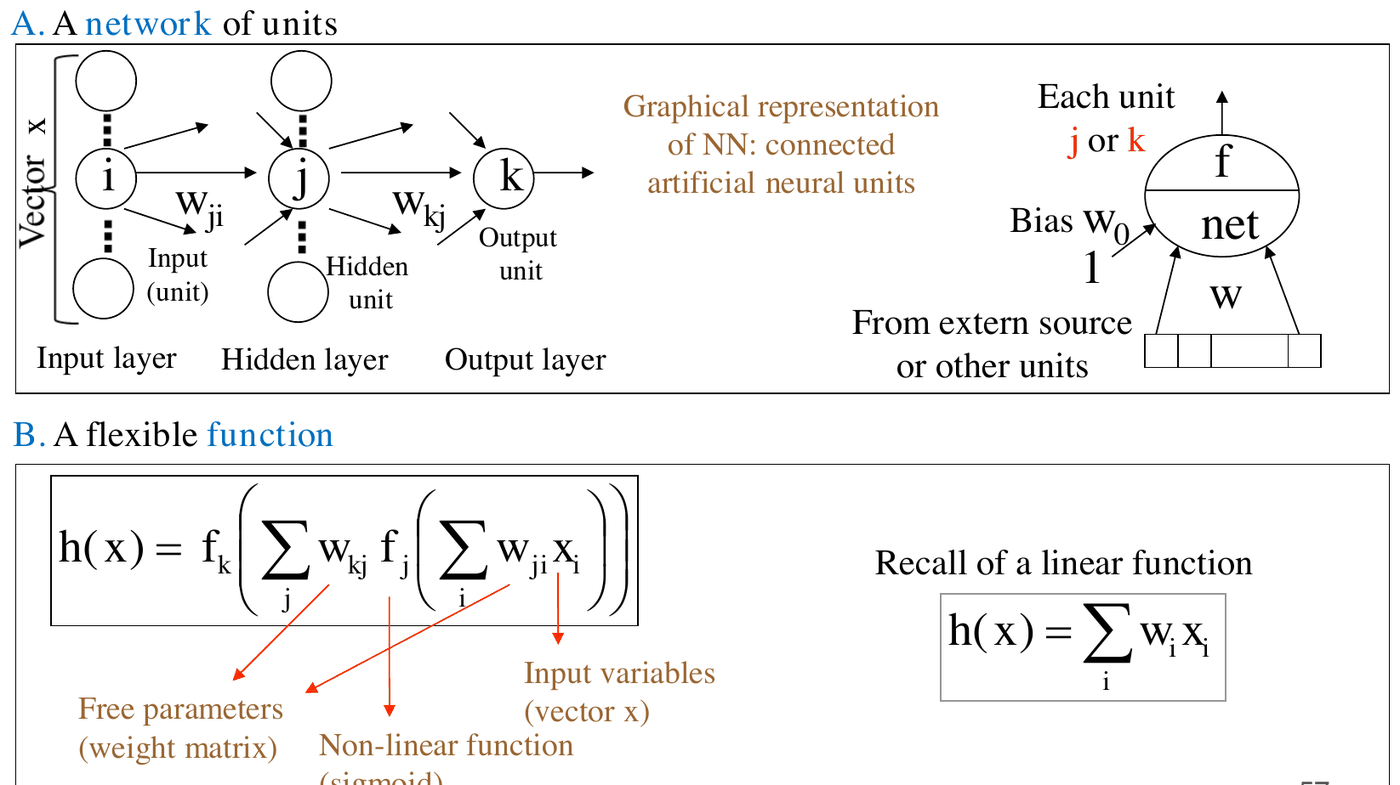
\includegraphics[width=0.91\linewidth,height=0.42\textheight,keepaspectratio]{images/06-nn1_due-viste.png}
\caption{The two views of a feedforward network with one hidden layer:
network of units (A) and flexible function (B).}
\end{figure}

\subsection{View A: a network of
units}\label{vista-a-una-rete-di-unituxe0}

In an MLP architecture:

\begin{itemize}
\tightlist
\item
  units are connected by weighted links and organised in
  \textbf{layers};
\item
  the \textbf{input layer} is just the source of the input
  \(\mathbf{x}\): it loads (copies) the pattern, without computing
  \(net\) or \(f\);
\item
  the \textbf{hidden layer} projects onto the output layer (or onto
  another hidden layer);
\item
  the \textbf{output layer} produces \(h(\mathbf{x})\).
\end{itemize}

\subsection{View B: a flexible
function}\label{vista-b-una-funzione-flessibile}

A two-layer network (one hidden and one output layer) computes \[
h(\mathbf{x}) = f_k\left(\sum_j w_{kj}\, f_j\left(\sum_i w_{ji}\, x_i\right)\right),
\] where \(x_i\) are the input variables, \(w\) the free parameters
(weight matrices) and \(f\) non-linear functions (sigmoids). Compare
with the linear function \(h(\mathbf{x}) = \sum_i w_i x_i\): the
network is a composition of linear and non-linear functions.

\subsection{Components of a neural
network}\label{componenti-di-una-rete-neurale}

A network is traditionally described by:

\begin{itemize}
\tightlist
\item
  the type of \textbf{unit} (net and activation function);
\item
  the \textbf{architecture} (number of units, topology, number of
  layers);
\item
  the \textbf{learning algorithm}.
\end{itemize}

\subsection{Uniform notation for
units}\label{notazione-uniforme-per-le-unituxe0}

For a generic unit \(t\) (which can be hidden, \(j\), or output,
\(k\)): \[
net_t(\mathbf{x}) = \sum_u w_{tu}\, o_u, \qquad o_t(\mathbf{x}) = f_t\big(net_t(\mathbf{x})\big),
\] where \(u\) denotes a generic input source (which can be \(i\) or
\(j\)). By loading the pattern into the input layer, the symbol \(o\)
can be used both for the inputs and for the outputs of the hidden
units: the input to unit \(t\) from source \(u\) (through the
connection \(w_{tu}\)) is \(o_u\). This notation will be used in the
derivation of backpropagation.

\begin{boxexample}{Exercise (from the lecture)}

\begin{enumerate}
\def\labelenumi{\arabic{enumi}.}
\tightlist
\item
  For the weights \(w_{ji}\) (input → hidden), the input \(o_u\) is
  \(o_i = x_i\), the component of the pattern.
\item
  For the weights \(w_{kj}\) (hidden → output), the input \(o_u\) is
  \(o_j\), the output of hidden unit \(j\).
\item
  \(w_{t0}\) is the \textbf{bias} of each unit \(t\), with constant
  input \(o_0 = 1\).
\item
  Hidden unit: \(o_j = f_j\left(\sum_i w_{ji}\,x_i\right)\); output
  unit: \(o_k = f_k\left(\sum_j w_{kj}\,o_j\right)\).
\end{enumerate}

\end{boxexample}

\subsection{Architecture and feedforward
processing}\label{architettura-e-processing-feedforward}

The \textbf{architecture} defines the connection topology. The
two-layer network described above is the standard, \textbf{fully
connected} MLP; there can be several hidden layers and also
connections that ``skip'' layers.

\begin{figure}[htbp]
\centering
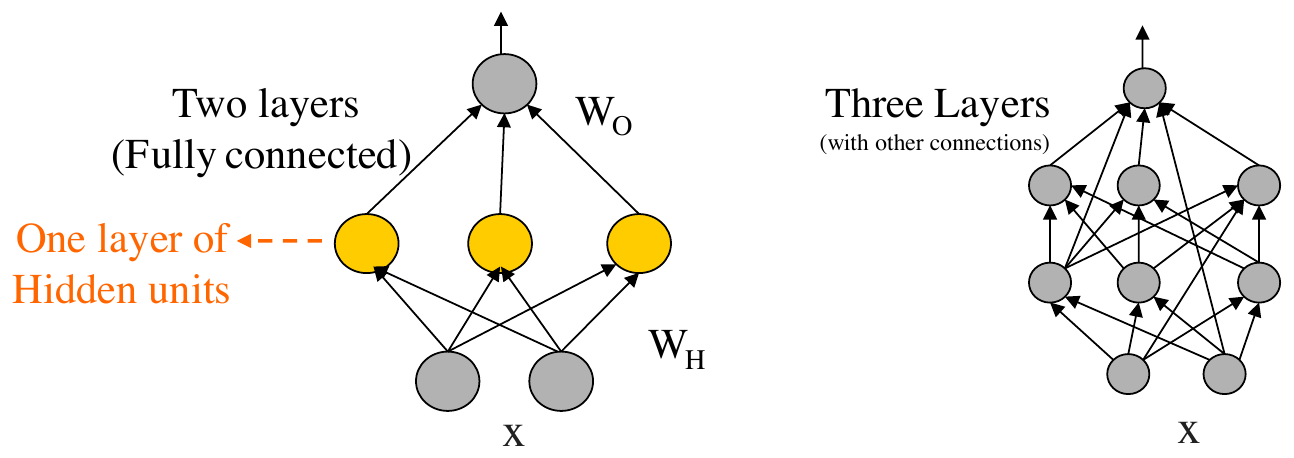
\includegraphics[width=0.71\linewidth,height=0.42\textheight,keepaspectratio]{images/06-nn1_architettura.png}
\caption{MLP architectures: two fully connected layers (left), three
layers with other connections (right).}
\end{figure}

The \textbf{feedforward} processing of a pattern proceeds from input to
output:

\begin{enumerate}
\def\labelenumi{\arabic{enumi}.}
\tightlist
\item
  the pattern \(\mathbf{x}\) is loaded into the input layer;
\item
  the outputs of all units of the first hidden layer are computed;
\item
  then those of the second hidden layer, and so on;
\item
  the outputs of the output layer are computed, i.e.\
  \(h(\mathbf{x})\);
\item
  the error (delta) at the output can now be computed.
\end{enumerate}

\begin{boxnote}{Recurrent networks}

\textbf{Feedforward} networks have a single direction input → output.
\textbf{Recurrent networks} add feedback connections (cycles):
self-loops give the network dynamic properties and a \textbf{memory}
of past computations, extending the model to the processing of
\textbf{sequences} (and structured data). They will be covered in a
dedicated lecture.

\end{boxnote}

\section{Why neural networks are
flexible}\label{perchuxe9-le-reti-neurali-sono-flessibili}

Three questions guide the analysis: why are networks a flexible model
(and can they be seen as LBE)? Is the flexibility theoretically
founded? How are the weights learned?

\subsection{Which tasks}\label{quali-task}

The hypothesis space is the \textbf{continuous space of all functions}
that can be represented by assigning values to the weights of a given
architecture. Depending on the output units, the network handles:

\begin{itemize}
\tightlist
\item
  \textbf{classification}, with sigmoidal output;
\item
  \textbf{regression}, with linear output.
\end{itemize}

With \textbf{multiple output units} one obtains multiple regression or
multi-class classifiers (for example three outputs giving
\(0.2;\ 0.7;\ 0.1\) for three classes).

\begin{figure}[htbp]
\centering
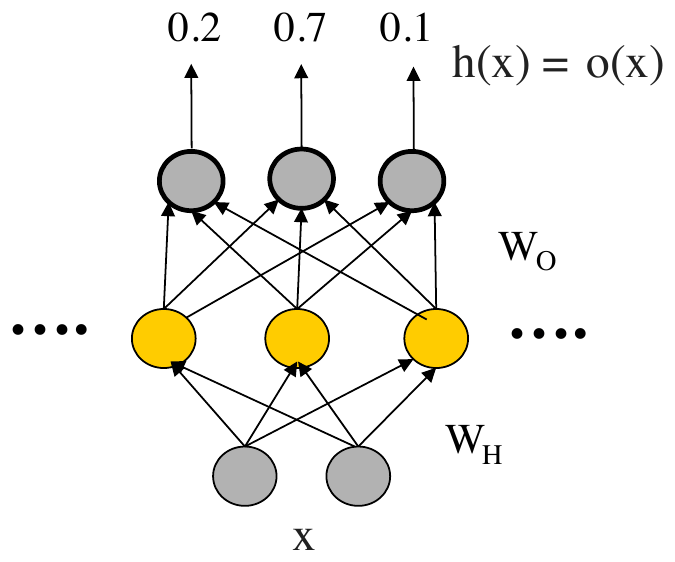
\includegraphics[width=0.37\linewidth,height=0.42\textheight,keepaspectratio]{images/06-nn1_multi-output.png}
\caption{A network with multiple outputs for a multi-class problem.}
\end{figure}

\subsection{The network as an adaptive basis
expansion}\label{la-rete-come-espansione-in-basi-adattiva}

The network computes
\(h(\mathbf{x}) = f_k\left(\sum_j w_{kj}\,f_j\left(\sum_i w_{ji}x_i\right)\right)\).
Units and architecture are just a graphical representation of the data
flow. Each term \[
\phi_j(\mathbf{x}, \mathbf{w}) = f_j\left(\sum_i w_{ji}\,x_i\right)
\] can be seen as computed by an independent hidden unit, or as a
\textbf{basis function \(\phi\) of an LBE}. Let us compare:

\begin{itemize}
\tightlist
\item
  \textbf{LBE}: \(h(\mathbf{x}) = \sum_j w_j\,\phi_j(\mathbf{x})\)
  (regression) or
  \(h(\mathbf{x}) = f\left(\sum_j w_j\,\phi_j(\mathbf{x})\right)\)
  (classification), with the \(\phi\) \textbf{fixed a priori} and the
  model linear in the parameters.
\item
  \textbf{Neural network}:
  \(h(\mathbf{x}) = f_k\left(\sum_j w_{kj}\,\phi_j(\mathbf{x}, \mathbf{w})\right)\),
  where now \textbf{the \(\phi\) depend on the weights} and therefore
  \textbf{adapt to the data} during training.
\end{itemize}

\begin{boxtip}{Neural networks as adaptive bases}

Neural networks are an \textbf{adaptive basis function} approach: the
bases themselves are adapted to the data (by learning the
\(\mathbf{w}\) inside the \(\phi\)). All bases are of the same type
(given by the activation function). \(h(\mathbf{x})\) is a non-linear
function of weighted sums of non-linearly transformed linear models,
with the crucial improvement of \textbf{adaptivity}. (To be compared
later with SVMs, another form of LBE.)

\end{boxtip}

Each hidden unit computes a new \textbf{non-linear derived feature}, in
an adaptive way. In other words: the representational capacity of the
model is tied to the presence of a \textbf{hidden layer with non-linear
activations}, which transforms the input into the \textbf{internal
representation} of the network. Learning defines a suitable internal
representation, i.e.\ new hidden features of the data, which allow the
model to extract the \textbf{higher-order statistics} relevant for
approximating the target function.

\begin{boxwarning}{Hidden units must be non-linear}

An MLP with \textbf{linear} units is equivalent to a \textbf{single
layer} network: the composition of linear functions is linear. With
\(f\) the identity,
\(h(\mathbf{x}) = \sum_j w_{kj}\sum_i w_{ji}x_i = \sum_i\left(\sum_j w_{kj}w_{ji}\right)x_i = \sum_i w'_i x_i\).

The price of non-linearity: the model is \textbf{non-linear in the
parameters} \(\mathbf{w}\), and training becomes a \textbf{non-linear
optimisation} (non-convex) problem.

\end{boxwarning}

\subsection{Universal
approximation}\label{lapprossimazione-universale}

\begin{boxtheorem}{Universal approximation theorem (Cybenko 1989, Hornik et al.)}

A network with \textbf{a single hidden layer} (with logistic
activations) and linear output can approximate arbitrarily well
\textbf{any continuous function} (on hypercubes), provided there are
enough hidden units: given \(f\) and \(\varepsilon > 0\), there exists
\(h\) such that \(|f(\mathbf{x}) - h(\mathbf{x})| < \varepsilon\) for
all \(\mathbf{x}\) in the hypercube. More generally, an MLP can
approximate arbitrarily well any input-output mapping, with enough
hidden units.

\end{boxtheorem}

(It can be thought of as a generalisation of approximation with finite
Fourier series.)

\begin{boxwarning}{It is an existence theorem}

The theorem says that the network \textbf{exists}, but it provides
neither the \textbf{algorithm} to find it nor the \textbf{number of
units} needed.

\end{boxwarning}

Two fundamental questions therefore remain: \textbf{how to learn}
(backpropagation, next lecture) and \textbf{how to choose the
architecture}.

\subsection{Expressive power and
VC-dimension}\label{potere-espressivo-e-vc-dimension}

The expressive power of a network depends on the \textbf{number of
units} and on their \textbf{configuration}. The number of units is
related to the VC-dimension: the capabilities of the network depend on
the number of parameters (in a fully connected MLP, roughly the number
of inputs times the number of hidden units, plus the hidden units times
the outputs), but also on the \textbf{value} of the weights:

\begin{itemize}
\tightlist
\item
  weights \(= 0\) → minimal VC-dim;
\item
  small weights → we work in the linear part of the sigmoid → small
  VC-dim;
\item
  large weights → more complex model.
\end{itemize}

Since training starts from weights close to 0 and the weights grow
during training, the network is a \textbf{variable-dimension hypothesis
space}: the effective VC-dim grows during learning. (This will be the
basis of \emph{early stopping}.)

\subsection{How many layers?
(preview)}\label{quanti-strati-anticipazione}

The universal approximation theorem says that one hidden layer is
enough, but it does not guarantee that a \textbf{small} number of units
is enough. There are ``\emph{no flattening}'' results (on efficiency,
not on expressiveness): functions that with a single hidden layer
would require an \textbf{exponential} number of units (with respect to
the input dimension), while with more layers far fewer are needed. But
is it easy to train an MLP with many layers? We will see it in deep
learning.

\subsection{The inductive bias of neural
networks}\label{il-bias-induttivo-delle-reti-neurali}

For networks trained with backpropagation, the inductive bias is
related to the \textbf{smoothness} properties of functions: small
changes in the input produce small changes in the output (for example,
locally bounded first derivative). It is a very common assumption in
ML, and it is reasonable: if the target function is not smooth (for
example a random number generator), generalisation is impossible
anyway.

\section{Towards the learning
algorithm}\label{verso-lalgoritmo-di-apprendimento}

The learning algorithm adapts the weights of the network to obtain the
best approximation of the target function, minimising as always an
error (or loss) function on the training data.

\subsection{The credit assignment
problem}\label{il-problema-del-credit-assignment}

\begin{itemize}
\tightlist
\item
  The Perceptron has a learning algorithm, but it does not represent
  all Boolean functions.
\item
  A network of perceptrons represents every Boolean function, but an
  algorithm is needed to train it.
\end{itemize}

What changes? The \textbf{credit assignment problem}: how much
``responsibility'' for the error should be attributed to the hidden
units? For the output units we know the desired response and hence the
error; for the hidden units \textbf{we do not know what their output
should be}, so the error signal is not directly measurable. Moreover,
the model is non-linear in the weights.

Minsky and Papert (1969) considered the problem too difficult; it was
solved by several researchers with the \textbf{backpropagation}
algorithm, popularised by Rumelhart, Hinton and Williams in the
\emph{PDP} book (1986): it was the \textbf{renaissance} of neural
networks.

\subsection{The loading problem}\label{il-loading-problem}

\begin{boxdefinition}{Loading problem}

Given a network and a set of examples, does there exist a set of
weights for which the network is consistent with the examples?
(``Loading'' the training data into the free parameters of the
network.)

\end{boxdefinition}

The loading problem is \textbf{NP-complete} (Judd, 1990): no polynomial
algorithm is known. In practice, however, networks are trained in
reasonable time with backpropagation, even though the optimal solution
is not guaranteed.

\subsection{The key idea: extending gradient
descent}\label{lidea-chiave-estendere-la-discesa-del-gradiente}

Gradient descent minimising a loss \textbf{extends to MLPs}, provided
that the loss and the activation functions are
\textbf{differentiable}: the task is to find the delta for
\textbf{every} unit of the network. The problem remains the same: given
\(l\) examples \((\mathbf{x}_p, d_p)\) and a loss \(L\) (for example
\(L(h(\mathbf{x}_p), d_p) = (d_p - h_\mathbf{w}(\mathbf{x}_p))^2\)),
find \(\mathbf{w}\) minimising \[
E(\mathbf{w}) = R_{emp} = \frac{1}{l}\sum_{p=1}^{l}\big(d_p - h(\mathbf{x}_p)\big)^2
\] by computing its gradient. We need: a differentiable loss,
differentiable activations and a network to follow the flow of
information.

Properties of backpropagation:

\begin{itemize}
\tightlist
\item
  it is simple thanks to the \textbf{compositional form} of the model;
\item
  it uses only quantities \textbf{local} to each unit, preserving
  modularity;
\item
  it is \textbf{efficient}: \(O(\#W)\) instead of \(O(\#W^2)\), thanks
  to the factorisation of the deltas;
\item
  regarding biological plausibility the debate is open (it has been
  hypothesised that the brain uses a sub-optimal local approximation of
  BP).
\end{itemize}

The full derivation is in the next lecture (and in the notes
\href{07\%20-\%20Note\%20sulla\%20backpropagation}{07 - Notes on
backpropagation}).

\subsection{Practical issues in
training}\label{questioni-pratiche-nelladdestramento}

The model is often \textbf{over-parameterised} and the optimisation is
\textbf{non-convex} and potentially unstable. The issues to address
(after backpropagation) are: initial weight values, learning rate,
on-line/batch; overfitting and regularisation; input scaling and output
representation; number of hidden units; multiple minima; stopping
criteria.

\begin{boxabstract}{Summary}

The artificial neuron computes \(o = f(\sum_j w_j x_j)\). The
\textbf{Perceptron} (threshold) has a learning algorithm that
\textbf{converges in a finite number of steps} for linearly separable
problems, but it does not represent XOR. Two-layer perceptron networks
represent every Boolean function thanks to the \textbf{internal
re-representation} of the hidden layer. Replacing the threshold with a
differentiable \textbf{sigmoid}, gradient descent can be used. The
\textbf{MLP} is a nested function
\(h(\mathbf{x}) = f_k(\sum_j w_{kj} f_j(\sum_i w_{ji} x_i))\),
interpretable as an \textbf{adaptive basis expansion}, and it is a
\textbf{universal approximator}. To train it, the \textbf{credit
assignment} of the hidden units must be solved: backpropagation does
this.

\end{boxabstract}

\begin{boxquestion}{Possible exam questions}

\begin{itemize}
\tightlist
\item
  Describe the artificial neuron and the main activation functions.
\item
  How are AND, OR, NOT represented with a perceptron? How is XOR
  solved?
\item
  Write the Perceptron learning algorithm.
\item
  State and prove the Perceptron convergence theorem.
\item
  Differences between the Perceptron algorithm and LMS; why can LMS
  fail on separable problems?
\item
  Derive the update rule for a single sigmoidal unit.
\item
  Why must hidden units be non-linear?
\item
  In what sense is a neural network an adaptive LBE?
\item
  State the universal approximation theorem and discuss its limits.
\item
  What is the credit assignment problem? And the loading problem?
\end{itemize}

\end{boxquestion}
